\documentclass[review]{siamart190516}

% 1. Preamble and packages
\usepackage{lipsum}
\usepackage{amsfonts}
\usepackage{graphicx}
\usepackage{epstopdf}
\usepackage{algorithmic}
\ifpdf%
  \DeclareGraphicsExtensions{.eps,.pdf,.png,.jpg}
\else
  \DeclareGraphicsExtensions{.eps}
\fi
\usepackage{amsopn}
\DeclareMathOperator{\diag}{diag}
\usepackage{booktabs}
\usepackage{bbm}
\usepackage{bm}
\usepackage{caption}
\usepackage{subcaption}
\usepackage[utf8]{inputenc}
\usepackage[T1]{fontenc}

\newcommand{\norm}[1]{\left\lVert#1\right\rVert}
\newcommand{\normtwo}[1]{\left\lVert#1\right\rVert_2}
\newcommand{\abs}[1]{\left\lvert#1\right\rvert}
\newcommand{\mat}[1]{\bm{{#1}}}
\renewcommand{\vec}[1]{\bm{{#1}}}
\newcommand{\lequiv}{\Leftrightarrow}
\newcommand{\bigO}[1]{\mathcal{O}\!\left(#1\right)}
\newcommand{\ceil}[1]{\left\lceil #1 \right\rceil}
\newcommand{\floor}[1]{\left\lfloor #1 \right\rfloor}
\newcommand{\sfrac}[2]{#1/#2}
\newcommand{\hquad}{\enskip}
\newcommand{\expected}[1]{\mathbb{E}\left[#1\right]}
\newcommand{\mspan}[1]{\text{span}\left( #1 \right)}
\newcommand{\prob}[1]{P\left(#1\right)}
\newcommand{\probt}[1]{P\left( \text{#1} \right)}
\newcommand{\condprob}[2]{P\left(#1 \:|\: #2\right)}
\newcommand{\condprobt}[2]{P\left(\text{#1} \:|\: \text{#2}\right)}
\newcommand{\bayes}[2]{\frac{\condprob{#2}{#1}\prob{#1}}{\prob{#2}}}
\newcommand{\bayesx}[3]{\frac{\condprob{#2}{#1}\prob{#1}}{\condprob{#2}{#1}\prob{#1} + \condprob{#2}{#3}\prob{#3}}}
\newcommand{\sech}{\text{sech}}
\newcommand*{\vertbar}{\rule[-1ex]{0.5pt}{2.5ex}}
\newcommand*{\horzbar}{\rule[.5ex]{2.5ex}{0.5pt}}
\newcommand{\vect}[2]{\underline{{#1}}_{{#2}}}
\newcommand{\basisp}[1]{\underline{{p}}_{{#1}}}
\newcommand{\basisq}[1]{\underline{{q}}_{{#1}}}
\newcommand{\coeff}[1]{\underline{{a}}_{{#1}}}
\newcommand{\bestfit}{\underline{\bar{x}}}
\newcommand{\grad}{\nabla}
\newcommand{\laplace}{\Delta}

% 2. Paper title
\newcommand{\TheTitle}{%
  A Supervised Learning Approach to Predicting Multigrid Convergence
}

% 2.5. Short title for running heads (if needed)
\newcommand{\TheShortTitle}{%
  \TheTitle
}

% 3. Student Name
\newcommand{\TheName}{Nicolas Nytko}

% 4. Student Address
\newcommand{\TheAddress}{%
  University of Illinois at Urbana-Champaign,
  (\email{nnytko2@illinois.edu}).
}

% 5. Acknowledge funding or other resources
\newcommand{\TheFunding}{%
  This work was funded by IJK\@.
}

% 6. Collaborators, such as advisor or research collaborators
\newcommand{\TheCollaborators}{%
  Matthew West,
  Luke Olson,
  Scott MacLachlan
}

% ---------------------------------------------
% ---------------------------------------------
\author{\TheName\thanks{\TheAddress}}
\title{{\TheTitle}}
\headers{\TheShortTitle}{\TheName}
\ifpdf%
\hypersetup{%
  pdftitle={\TheTitle},
  pdfauthor={\TheName}
}
\fi

\begin{document}

\maketitle

\begin{center}
In collaboration with:
  {\TheCollaborators}
\end{center}
\vspace{1cm}
% ---------------------------------------------
% ---------------------------------------------

\begin{abstract}
  \input{../abstract/abstract.txt}
\end{abstract}

\begin{keywords}
  convergence, relaxation weight, machine learning, supervised learning, graph net, cnn, convolutional network
\end{keywords}

\section{Introduction}\label{sec:intro}

Multigrid methods are some of the most widely used linear solvers for sparse systems, particularly ones that arise from the discretization of partial differential equations.  By ``downsampling'' the original problem to a series of smaller and smaller problems, fast convergence can be obtained with minimal work\cite{mgtut}.  The question becomes, what is the optimal way to downsample each problem and obtain a splitting of coarse/fine points?  Classical Algebraic Multigrid (AMG) techniques attempt to answer this by exploiting the structure of the original system to create a set of interpolation operators\cite{rs}.  However, these methods often require careful parameter tweaking to obtain sensible splittings and often the best way to test the parameter space is to actually run the multigrid iterations.

In this paper, a method of training neural networks to predict convergence rates for a specific PDE or class of equations is introduced.  The neural networks take as input a C/F splitting of a mesh, the output of an AMG aggregation/splitting method, and give a rate of convergence between $0$ and $1$, inclusive.  Lower values of convergence indicate faster methods -- more of the error is dissipated at each iteration.  Two problems are discussed here: $(1)$ a 1D variable coefficient Poisson equation, and $(2)$ a 2D recirculating flow convection-diffusion problem with specific parameters.  Sections \ref{subsec:methods_poisson} and \ref{subsec:methods_conv} describe how random grid splittings are generated for the two problems and evaluated in a multigrid solver.

For the 1D poisson case, convolutional neural networks (CNNs) are trained to predict the convergence rate and optimal relaxation weight (Section \ref{subsec:poisson_cnn}).  For the 2D convection-diffusion problem, a CNN was first trained to predict convergence (Section \ref{subsec:conv_cnn}), and then two different graph nets were trained to extrapolate to differently sized inputs and non-grid meshes (Sections \ref{subsec:conv_gcn}, \ref{subsec:conv_mpnn}).  Numerical results consisting of the network error performance and sample predictions are shown in Section \ref{sec:num}.  Finally, further discussion and possible directions of future work are given in Section \ref{sec:conc}.

\section{Methods}\label{sec:methods}

The methods described here will be split into two subsections describing each problem that was explored. First, the Poisson case and the data generation is discussed (Section \ref{subsec:methods_poisson}) followed by the respective convolutional neural network that was trained (Section \ref{subsec:poisson_cnn}).  Afterwards, an overview of the data generation for the 2D convection-diffusion problem is given (Section \ref{subsec:methods_conv}) and then followed by a description of the convolutional network that was trained (Section \ref{subsec:conv_cnn}).  The use of two graph nets is also described: one that performs a simple edge convolution for each node (Section \ref{subsec:conv_gcn}), and another that implements ``message passing'' and learns optimal edge weighting of the convolution (Section \ref{subsec:conv_mpnn}).

\subsection{1D Poisson}\label{subsec:methods_poisson}

Formally, the problem being solved is the Poisson equation in one dimension with variable coefficients
%
\begin{equation} \label{eqn:poisson}
  -\grad \cdot \left(k\left(\vec{x}\right) \grad\vec{u}\right) = f,
\end{equation}
%
with the right-hand side $f\left(\vec{x}\right)=\vec{x}$ being arbitrarily chosen.  Eqn.~\eqref{eqn:poisson} is discretized using finite differences on a grid of $N=31$ internal points on the domain $\Omega = \left[-1, 1\right]$ and Dirichlet boundary conditions, $\partial\Omega = 0$.  To preserve the symmetric, positive definite properties of the resulting linear system, the $k\left(\vec{x}\right)$ function is discretized on the grid \textit{midpoints}\cite{numpde}.

Before the neural network can be trained, a dataset of approximately 300,000 random C/F grid splittings and their computed convergence rate and optimal relaxation weight was generated.  A set of $6$ reference grids were first created according to various ``coarsening'' factors:
%
\begin{equation} \label{eqn:poisson_coarsening}
  r = \begin{Bmatrix} 2 & 3 & 4 & 5 & 6 & 7 & 8 & 9\end{Bmatrix}.
\end{equation}
%
Each of the values in \ref{eqn:poisson_coarsening}, say $r_i = j$ refers to a grid in which each $j$th point is coarse, and the rest fine.  So, a coarsening by $3$ is a grid that has roughly $\frac{1}{3}$ of its distribution of points as coarse and all others fine.  Each of these reference grids was randomly permuted such that each grid point had a random probability of being flipped to the opposite value -- coarse point to fine and fine point to coarse.  For each reference grid, approximately 1000 random trials of each following probability were run:
%
\begin{equation} \label{eqn:poisson_probabilities}
  p = \begin{Bmatrix} 0.01 & 0.05 & 0.1 & 0.25 & 0.5 & 0.75 \end{Bmatrix}
\end{equation}
%
Additionally, each trial was run with a randomly-chosen function for the variable coefficients $k\left(\vec{x}\right)$.  The function is randomly chosen from
%
\begin{equation} \label{eqn:poisson_varcoefficients}
k\left(\vec{x}\right) = \begin{cases}
\alpha & 0 < \alpha < 10 \\
\text{rand()}\left(\alpha + 1\right) & 0 < \alpha < 10 \\
\alpha\cos\left(\pi x \beta\right) + \gamma & 0 < \alpha < 10, 0 < \beta < 10, \alpha < \gamma < 10\\
\abs{\sum_{i=1}^5 \alpha_i x^i} + 0.01 & -10 < \alpha < 10
\end{cases},
\end{equation}
%
with coefficient values specifically picked to prevent the function from being non-positive at any value in $\Omega$.

The full set of C/F splittings was then given to a 2 level V-cycle Multigrid solver that was run for a maximum of 15 iterations.  The solver is composed of one round of weighted Jacobi pre-smoothing, a coarse error correction, then another round of Jacobi post-smoothing.  At each iteration, the absolute error between the approximation and the ``exact'' solution (pre-computed via sparse linear solve) was found and saved: $e_i = \norm{\mat{A}^{-1}\vec{f} - \vec{u}_i}$.  This sequence of errors was then used to compute the average convergence rate.  To acquire the optimal relaxation weight, the smoother was run through a bracketed numerical optimization method with the assumption that the convergence rate is unimodal as a function of relaxation weight. \footnote{Experimental testing generally asserts this to be true, however this will remain a conjecture for now.}

\subsection{Poisson CNN}\label{subsec:poisson_cnn}

Two separate deep convolutional networks with residual connections were trained to separately predict the optimal relaxation weight and convergence rate when given a linear C/F splitting.  The architecture for both networks is identical and a textual overview is given here:
%
\begin{enumerate}
\item 6 1D CNN layers of kernel size 7, input 2 channels output 7 channels.  Padding by three on each side to keep dimensions static.
\item 6 CNN layers of kernel size 5, input/output 7 channels.  Padding by two on each side.
\item 6 CNN layers of kernel size 3, input/output 7 channels.  Padding by 1 on each side.
\item Max-pooling layer of kernel 2, stride 2.  Effectively reduces input size by half.
\item 8 Fully-connected layers to gradually reduce output to a scalar describing the convergence or relaxation weight.
\end{enumerate}
%
Each layer is followed by an implicit ReLU nonlinear activation function.  Because the convolutional layers (except for the first) keep the input and output size static, we are able to push residual values and skip layers similarly to a ResNet\cite{huang2018densely,he2015deep}.  Even numbered layers $n$ take as input both the output of layers $n-1$ and $n-2$, while odd-numbered layers only use the output from layer $n-1$.

The C/F splitting is remapped such that a coarse point is given a value of $1$ and a fine point the value of $-1$.  The variable coefficients were also re-discretized to be defined on the nodal points instead of midpoints in order for the splitting and coefficients to be represented by vectors of same length.  These two were then stacked into a two-channel tensor for input into the CNN.  When training, input values (convergence rate and relaxation weight) are normalized to be within the range of $\left[0,1\right]$.  This normalization is undone when the output is displayed.

\subsection{2D Convection-Diffusion}\label{subsec:methods_conv}

This specific problem models what is called the \textit{double glazing problem}, modeling the temperature distribution of a cavity with a single ``hot'' wall.  This is given by the differential equation:
%
\begin{equation}\label{eqn:conv}
  -k\grad^2u + \vec{w}\cdot\grad u = f.
\end{equation}
%
The wind velocity function, $\vec{w}\left(x,y\right)$ is defined as $\vec{w}\left(x,y\right)=\\ \begin{bmatrix} 2y\left(1-x^2\right) & 2x\left(1-y^2\right) \end{bmatrix}$.  The domain is a square of side length two centered at the origin, $\Omega = \left[-1,1\right] \times \left[-1,1\right]$.  Dirichlet boundary conditions are defined on $\partial \Omega$, with the one ``hot'' wall defined on $x=1$ with value $\partial \Omega_H=1$.  The other boundaries are ``cold'' walls with $\partial \Omega_c=0$.  A diffusivity constant of $k=0.1$ is used.  This problem is derived from an example by Elman, Silvester, and Wathen\cite{silvester}.

This PDE is discretized using finite-elements on a structured grid of 25x25 internal points using the Firedrake software for FEM discretizations\cite{Dalcin2011, Rathgeber2016,Homolya2016,McRae2016,MUMPS01,MUMPS02}.  Using a grid as a basis for the discretization allows use of both CNN and more sophisticated graph convolutional techniques.

Generating a dataset of mesh splittings and convergence rates was done in an overall similar way to the 1D Poisson equation with a few notable differences.  Again, a set of reference C/F splittings were generated that are later permuted.  For the convection-diffusion case, the following reference splittings were used:

\begin{enumerate}
\item All fine points
\item All coarse points
\item Splitting as given by Ruge-St\"{u}ben AMG ($\theta=0.25$) \cite{rs, pyamg}
\item Coarsening in each direction by 2
\item Coarsening in each direction by 3
\item Coarsening in each direction by 4
\item Coarsening in each direction by 5
\end{enumerate}

The entries of each individual reference splitting were then randomly permuted according to a defined probability.  The probability values used are the same as those in the Poisson case, repeated here for convenience:
%
\begin{equation} \label{eqn:conv_probabilities}
  p = \begin{Bmatrix} 0.01 & 0.05 & 0.1 & 0.25 & 0.5 & 0.75 \end{Bmatrix}.
\end{equation}
%
Generated splittings that are unsolveable (i.e., consist of no coarse points) were rejected and their trial re-run.  This generated set of C/F splittings was passed along to another 2 level V-cycle multigrid solver run for a maximum of 50 iterations.  The interpolation operator was formed by means of \textit{direct interpolation}, the implementation of which gratiously taken from the PyAMG\cite{pyamg} library.  This solver performs two rounds of Jacobi pre-and-post relaxation, with a coarse error correction between the relaxation steps.  The absolute error between the approximation at each iteration and the ``exact'' solution was computed and saved, with the full sequence used to find the average convergence rate.  Note the optimal Jacobi relaxation weight was not found here, as experimentation found that the optimal weight would nearly always be $1$.

The convection-diffusion problem was additionally re-discretized at 4 different mesh sizes: $15\times 15,\enskip 25\times 25,\enskip 35\times 35,\enskip 50\times 50$.  The above process was re-run for each mesh size to generate a new dataset for use in the graph nets.  To distinguish between the two datasets, they will hereby be referred to as the \textit{statically-sized} (only containing $25 \times 25$ mesh and splittings) and the \textit{variably-sized} datasets.

\subsection{Convection-Diffusion CNN}\label{subsec:conv_cnn}

A 2D convolutional network was trained on the statically-sized dataset to predict convergence when given a C/F splitting for the specific recirculating flow problem.  Since the input parameters are slightly less complex, a less deep (\textit{shallower}, if you will) network was trained:
%
\begin{enumerate}
\item 3 2D CNN layers of kernel 7, input two channels output 7 channels.  Padding by three on each side to keep dimensions.
\item 3 CNN layers of kernel 5, input/output 7 channels.  Padding by two on each side.
\item 3 CNN layers of kernel 3, input/output 7 channels.  Padding by 1 on each side.
\item 2D Max-pooling layer of kernel 2, stride 2.  Effectively reduces input size by half.
\item 1 Fully-connected layer to reduce output to a scalar predicting convergence rate.
\end{enumerate}
%
Each layer is followed by a ReLU nonlinear activation function.  Odd layers are fed the output of the previous two layers, while even layers are fed the input of only the previous layer, similarly to a ResNet\cite{huang2018densely,he2015deep}.  C/F splittings are mapped so that coarse points have value $1$ and fine points have value $-1$.  The CNN thus has a $25\times 25=625$-length vector as input.  Interestingly, normalization of the convergence rates is unneeded as the minimum and maximum recorded values are already close to $0$ and $1$, respectively.

\subsection{Convection-Diffusion Graph Convolutional Network (GCN)}\label{subsec:conv_gcn}

The main downside of using traditional convolutional layers is that they are useful only on structured, grid-like inputs.  Grid-based convolution is ineffective on the more complex meshes that may arise from finite-element discretizations.  By treating the input mesh as a graph and using graph-based convolution techniques, we may get around this roadblock.  The first graphnet that was tried uses the GCN layer introduced by Kipf and Welling\cite{gcn} and is described here, the other uses an Edge-Conditioned Convolution (ECC)/message passing layer and is described in Section \ref{subsec:conv_mpnn}.

For the graphnets, the sparse FEM system was re-interpreted as a graph by assigning each row/column to be a node and defining connectivity between nodes as nonzero matrix entries.  Edge weights were taken to be the entry values themselves, although normalized to be within the range of $[0, 1]$.   This network was trained on the variably-sized dataset; as will be seen, the lack of any fully-connected layers allows for any arbitrary input.

The Graph Convolutional Network (GCN) layer is defined as an operator on the graph Laplacian, using the following propagation rule:
%
\begin{equation}
  \mat{H}^{\left(i\right)} = \sigma\left( \mat{\tilde{D}}^{-\frac{1}{2}} \mat{\tilde{A}} \mat{\tilde{D}}^{-\frac{1}{2}} \mat{H}^{\left(i-1\right)} \mat{W}^{\left(i\right)} + \vec{b}^{(i)} \right).
\end{equation}
%
With $\mat{H}^{\left(i\right)}$ being the $i$'th hidden layer, $\mat{\tilde{A}} = \mat{A} + \mat{I}$ the adjacency matrix with added self loops, $\tilde{d}_{ii}=\sum_j\tilde{a}_{ij}$ a diagonal matrix consisting of the sum of outgoing edge weights, $\mat{W}^{(i)}$ the weight matrix at layer $i$, $\vec{b}^{(i)}$ a learned bias vector with same shape as $\mat{H}^{(i)}$, and $\sigma\left(\cdot\right)$ some nonlinear activation function.  Hidden layers have dimensions $n \times f$, with $n$ the number of graph nodes and $f$ the number of features at each node.  Thus, using only GCN layers it is not possible to reduce the number of rows in hidden layers (or the input layer for that matter).

Assume $\sigma\left(\cdot\right) = \text{ReLU}\left(\cdot\right) = \text{max}\left\{\cdot, 0\right\}$ for all activation functions.  Let $\mat{X}$ be the $n \times 1$ vector containing C/F splitting values for each node.  The network that was trained for this application consisted of the following architecture:
\begin{align*}
\mat{H}^{(1)} &= \sigma\left( \mat{D}^{-\frac{1}{2}} \mat{A} \mat{D}^{-\frac{1}{2}} \mat{X} \mat{W}^{(1)} + \vec{b}^{(1)} \right) \in \mathbb{R}^{n \times 2} \displaybreak[0] \\
\mat{H}^{(2)} &= \sigma\left( \mat{D}^{-\frac{1}{2}} \mat{A} \mat{D}^{-\frac{1}{2}} \mat{H}^{(1)} \mat{W}^{(2)} + \vec{b}^{(2)}\right) \in \mathbb{R}^{n \times 3} \displaybreak[0]\\
  \mat{H}^{(3)} &= \sigma\left( \mat{D}^{-\frac{1}{2}} \mat{A} \mat{D}^{-\frac{1}{2}} \mat{H}^{(2)} \mat{W}^{(3)} + \vec{b}^{(3)}\right) \in \mathbb{R}^{n \times 2} \displaybreak[0]\\
  \mat{H}^{(4)} &= \sigma\left( \mat{D}^{-\frac{1}{2}} \mat{A} \mat{D}^{-\frac{1}{2}} \mat{H}^{(3)} \mat{W}^{(4)} + \vec{b}^{(4)}\right) \in \mathbb{R}^{n \times 1} \displaybreak[0]\\
\mat{R} &=
\begin{bmatrix}
\hdots & \mat{X}^T & \hdots \\
\hdots & \left(\mat{H}^{(1)}\right)^T & \hdots \\
\hdots & \left(\mat{H}^{(2)}\right)^T & \hdots \\
\hdots & \left(\mat{H}^{(3)}\right)^T & \hdots \\
\hdots & \left(\mat{H}^{(4)}\right)^T & \hdots \\
\end{bmatrix} \in \mathbb{R}^{9 \times n} \displaybreak[0]\\
y &= \sum_{j=1}^n \sigma\left( \sigma\left(\mat{r}_j\mat{W}^{(5)} + \vec{b}^{(5)}\right) \mat{W}^{(6)} + \vec{b}^{(6)}\right) \in \mathbb{R}
\end{align*}

Note that the matrix $\mat{R}$ is formed whose columns are the propagation history of each node; this is an attempt to emulate traditional ResNet architectures.  The final scalar output is computed by summing each column of $\mat{R}$ through a two layer fully-connected neural network, with the first layer taking as input 9 features and outputting 5 features, and the second layer taking as input 5 features and outputting 1 feature.  This local transformation of each nodal value following by a global averaging removes any dependency for a fixed input size -- instead any sized graph and splitting could (in theory) be used.

\subsection{Convection-Diffusion Message Passing Network (MPNN)}\label{subsec:conv_mpnn}
A downside of the GCN layer, while being simple to implement and understand, is that it does not effectively learn edge features between nodes and thus is only an approximation of a convolution on a graph.  The Edge-Conditioned Convolution (ECC) layer, as defined by Simonovsky and Komodakis\cite{ecc}, attempts to combat this by learning optimal edge weights given an arbitrary node-edge neighborhood.  This approach is also referred to as a ``message-passing network'', as each connected neighbor attempts to learn a ``message'' that is passed to the original node\cite{mpnn}.  The convolution operation is defined as
%
\begin{equation}\label{eqn:mpnn_prop}
  \left(\mat{H}^{(i)}\right)_j = \frac{1}{\abs{\mathcal{N}\left(j\right)}} \sum_{k\in\mathcal{N}\left(j\right)} F^{(i)}\left(e_{j,k}\right)\left(\mat{H}^{(i-1)}\right)_k + \vec{b}^{(i)}
\end{equation}
%
where $\mat{H}^{\left(i\right)} \in \mathbb{R}^{n \times f_i}$ is the $i$'th hidden layer, $\mathcal{N}\left(i\right)$ is a map returning the neighborhood of vertex $i$ (including itself), $F^{(i)} \: : \: E \mapsto \mathbb{R}^{f_i \times f_{i-1}}$ is some function (in our case a small fully-connected neural network) that outputs a learned weight matrix given an edge, and $\vec{b}^{(i)}$ is a bias term for layer $i$.  The notation $\left(\mat{H}^{\left(i\right)}\right)_j$ here denotes the $j$'th row of the $i$'th hidden layer.

Using the ECC layer, another graph net was trained to predict the convergence rate given some C/F mesh splitting.  The architecture is identical to that in Section \ref{subsec:conv_gcn} with the exception that the propagation layers $\mat{H}^{(i)}: \hquad i=1\ldots 4$ are replaced with (\ref{eqn:mpnn_prop}) and surrounded with a ReLU activation layer.  Each $F^{(i)}$ is a two-layer fully-connected network taking some edge $\vec{e} \in \mathbb{R}^{f_i}$ and outputting a weight matrix $\mat{\Theta} \in \mathbb{R}^{f_i\times f_{i-1}}$.

% \section{Main Contribution}\label{sec:main}

\section{Numerical Results}\label{sec:num}

\begin{table}[t]
\centering
\begin{tabular}{|l|l|l|l|}
\hline
Model & Metric & Dataset & Value \\

\hline
Jacobi Weight & MSE & Training & $1.8331 \times 10^{-3}$ \\
Jacobi Weight & MSE & Testing & $1.8396 \times 10^{-3}$ \\
Jacobi Weight & L1 & Training & $2.9254 \times 10^{-2}$ \\
Jacobi Weight & L1 & Testing & $2.9271 \times 10^{-2}$ \\
\hline
Convergence Factor & MSE & Training & $1.4839 \times 10^{-3}$ \\
Convergence Factor & MSE & Testing & $1.5171 \times 10^{-3}$ \\
Convergence Factor & L1 & Training & $2.3908 \times 10^{-2}$ \\
Convergence Factor & L1 & Testing & $2.3865 \times 10^{-2}$ \\
\hline
\end{tabular}
\caption{Final training and testing Mean Squared Error (MSE)/$L^1$-norm loss values for the two Poisson models.  Lower values correspond to higher model accuracy.}
\label{tab:poisson_loss}
\end{table}

\subsection{1D Poisson}

A total of 336,000 C/F ``grid'' splittings were randomly generated for the variable-coefficient Poisson model.  Of these, a random 85\% of data items were designated as a training set and the remaining 15\% reserved for a testing set.  The relaxation and convergence CNNs were trained for a total of 30 epochs each, where each epoch is a total pass over all training set entries.  Models were trained using an MSE loss, and final loss values for both networks are detailed in Table \ref{tab:poisson_loss}.

Overall, the resulting data is encouraging and seems to indicate that both convergence factors and relaxation weights for the Poisson problem are predictable using a convolution-based network.  Sample convergence rate predictions on the training and testing subsets are shown in Figure \ref{fig:poisson_conv_pred}; these plots display predicted rates as a function of the true rates, so error is indicated by deviation from the diagonal of the plots.  It is interesting to visually see that the network has an easier time predicting more convergent grids ($c < 0.6$ or so) than more degenerate grids.  A lack of predictions less than $\approx 0.1$ is a deficiency of the input data not having grids with those convergence values.

Predictions for relaxation weights on both training and testing subsets are shown in Figure \ref{fig:poisson_jacobi_pred}.  Like the previous convergence plots, more accurate predictions are closer to the plot diagonals.  There is a positive correlation between the predictions and the true values, though unlike the convergence rates there is no obvious ``split'' in the prediction data.  The lack of predictions below $0.1$ is likely to also be caused by the input data.

\begin{figure}[h]
  \centering
  \begin{subfigure}{.48\textwidth}
    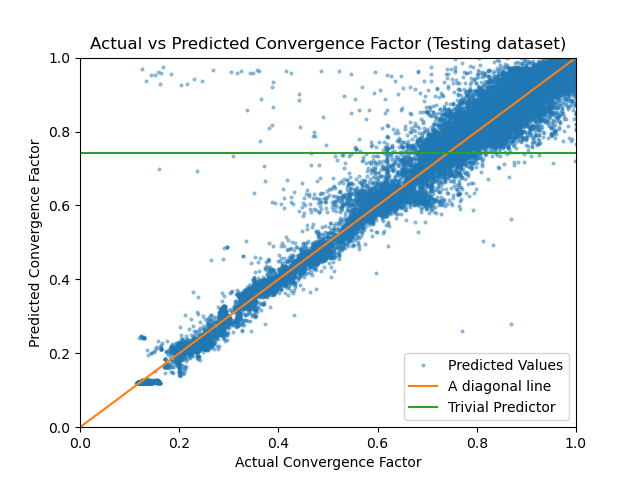
\includegraphics[width=\textwidth]{figs/poisson_conv_test_pred.png}
    \caption{Testing predictions}
    \label{subfig:poisson_conv_test}
  \end{subfigure}
  \begin{subfigure}{.48\textwidth}
    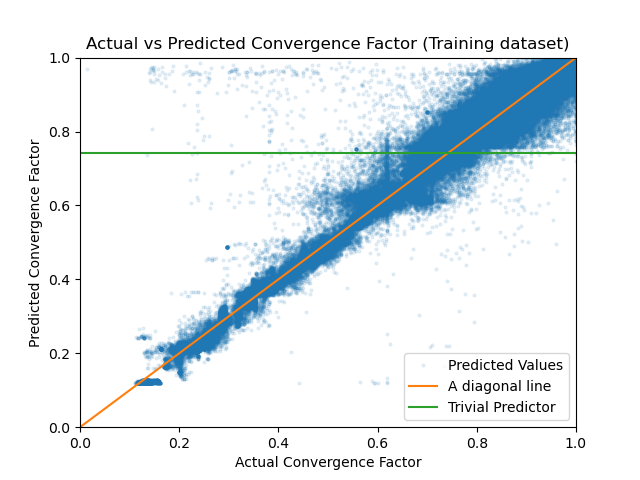
\includegraphics[width=\textwidth]{figs/poisson_conv_train_pred.png}
    \caption{Training predictions}
    \label{subfig:poisson_conv_train}
  \end{subfigure}
  \caption{Predicted convergence values vs. true convergence values on (\ref{subfig:poisson_conv_test}) testing and (\ref{subfig:poisson_conv_train}) training datasets for Poisson equation. Values closer to the diagonal represent more accurate predictions. }
  \label{fig:poisson_conv_pred}
\end{figure}

\begin{figure}[h]
  \centering
  \begin{subfigure}{.48\textwidth}
    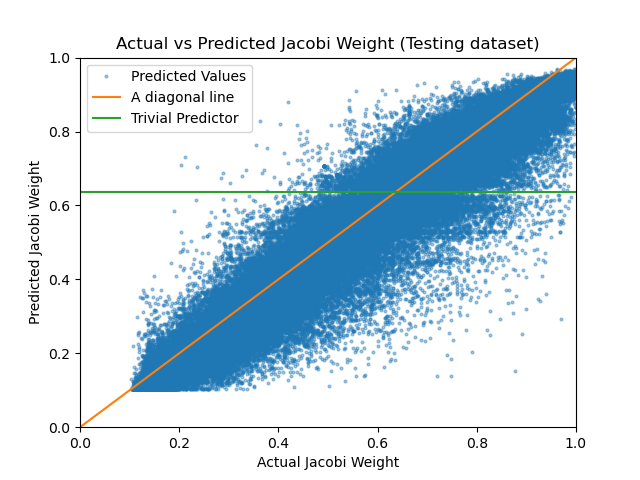
\includegraphics[width=\textwidth]{figs/poisson_jacobi_test_pred.png}
    \caption{Testing predictions}
    \label{subfig:poisson_jacobi_test}
  \end{subfigure}
  \begin{subfigure}{.48\textwidth}
    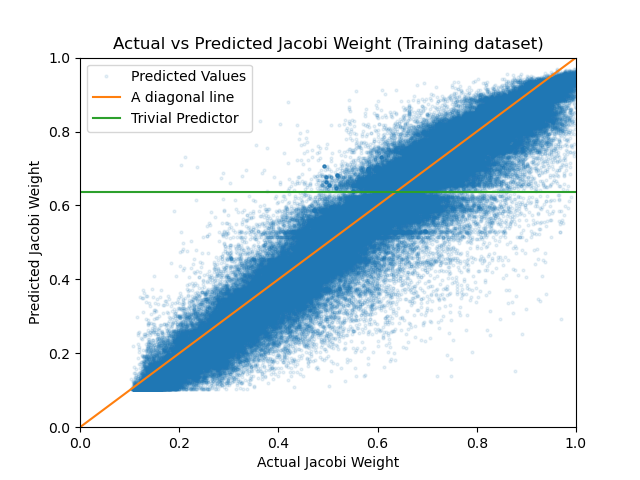
\includegraphics[width=\textwidth]{figs/poisson_jacobi_train_pred.png}
    \caption{Training predictions}
    \label{subfig:poisson_jacobi_train}
  \end{subfigure}
  \caption{ Predicted relaxation weights vs. true relaxation weights on (\ref{subfig:poisson_jacobi_test}) testing and (\ref{subfig:poisson_jacobi_train}) training datasets for Poisson equation. Values closer to the diagonal represent more accurate predictions. }
  \label{fig:poisson_jacobi_pred}
\end{figure}

\subsection{2D Convection-Diffusion}

Two datasets were created for the 2D recirculating flow problem: a set of \textit{statically-sized} C/F splittings and a set of \textit{variably-sized} splittings; both datasets consisted of $84,000$ elements.  The variably-sized dataset was evenly divided into the four mesh sizes: $15\times 15,\: 25\times 25,\: 35\times 35,\: 50\times 50$.  Each dataset was then split 85\%-15\% into training and testing subsets.  All neural networks were trained for 10 epochs each on an MSE loss, final loss values are detailed in Table \ref{tab:conv_loss}.  The recirculating flow CNN was trained and tested on the static dataset, while the two graph nets were trained on the variable dataset and evaluted on both datasets.

Again, results show that networks are able to learn convergence values for the particular multigrid solver and recirculating-flow problem.  Graph nets and convolutional networks seem to have more-or-less the same predictive power, with the graph nets having the obvious upside of being cable of handling non-grid inputs.  Interestingly enough, the GCN network had slightly better performance than the MPNN on the static dataset.  The opposite was true for the variable dataset, perhaps indicating the MPNN was able to generalize more overall.

\begin{table}[t]
\centering
\begin{tabular}{|l|l|l|l|}
\hline
Dataset & Model & Metric & Value \\
\hline
Static & CNN & MSE & $6.0332 \times 10^{-3}$ \\
Static & CNN & L1 & $5.2335 \times 10^{-2}$ \\
\hline
Static & GCN & MSE & $6.7278 \times 10^{-3}$ \\
Static & GCN & L1 & $5.5773 \times 10^{-2}$ \\
\hline
Static & MPNN & MSE & $8.4461 \times 10^{-3}$ \\
Static & MPNN & L1 & $7.0079 \times 10^{-2}$ \\
\hline
Variable & GCN & MSE & $1.3079 \times 10^{-2}$ \\
Variable & GCN & L1 & $8.4827 \times 10^{-2}$ \\
\hline
Variable & MPNN & MSE & $1.1495 \times 10^{-2}$ \\
Variable & MPNN & L1 & $7.9967 \times 10^{-2}$ \\
\hline
\end{tabular}
\caption{Final testing Mean Squared Error (MSE)/$L^1$-norm loss values for trained neural networks for the recirculating flow problem.  Lower values correspond to higher model accuracy.}
\label{tab:conv_loss}
\end{table}

Predicted convergence values by the CNN over the static dataset are displayed in Figure \ref{fig:cd_conv_pred}.  The subplots detail predicted convergence rates vs their true value for each C/F splitting.  Almost opposite to the phenomenon observed in the Poisson CNN (Figure \ref{fig:poisson_conv_pred}, the network predicts more poorly converging grids accurately.  This could perhaps be explained by the data more densely populated with the poor convergence grids, and has a distinct lack of optimal grids.

\begin{figure}[h]
  \centering
  \begin{subfigure}{.48\textwidth}
    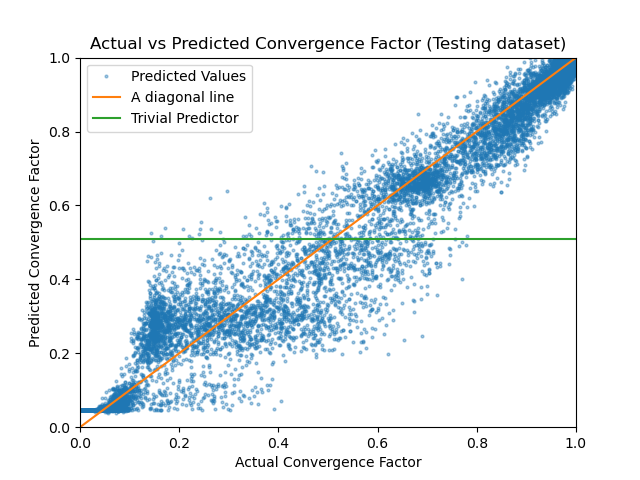
\includegraphics[width=\textwidth]{figs/cd_conv_test_pred.png}
    \caption{Testing predictions}
    \label{subfig:cd_conv_test}
  \end{subfigure}
  \begin{subfigure}{.48\textwidth}
    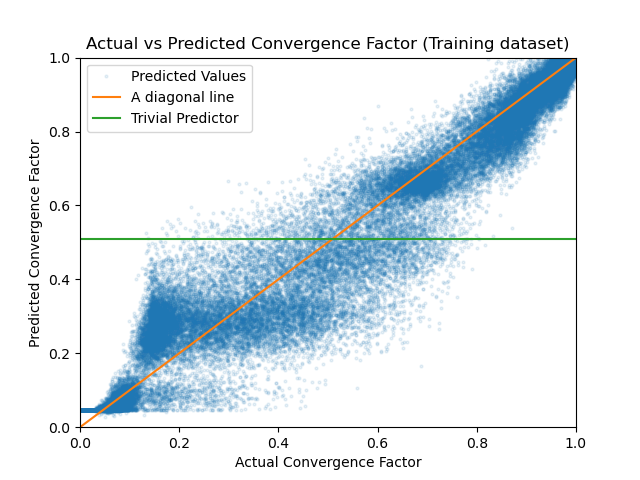
\includegraphics[width=\textwidth]{figs/cd_conv_train_pred.png}
    \caption{Training predictions}
    \label{subfig:cd_conv_train}
  \end{subfigure}
  \caption{Predicted convergence rates vs. true convergence rates on (\ref{subfig:cd_conv_test}) testing and (\ref{subfig:cd_conv_train}) training datasets for model convection-diffusion problem, using a convolutional network. Values closer to the diagonal represent more accurate predictions. }
  \label{fig:cd_conv_pred}
\end{figure}

Convergence predictions by the ECC network over the variable-size dataset are given in Figure \ref{fig:cd_mpnn_pred}.  Various horizontal trends of predictions are visible in the plots, with distinct subsets of convergence factors all being predicted as the same value.

\begin{figure}[h]
  \centering
  \begin{subfigure}{.48\textwidth}
    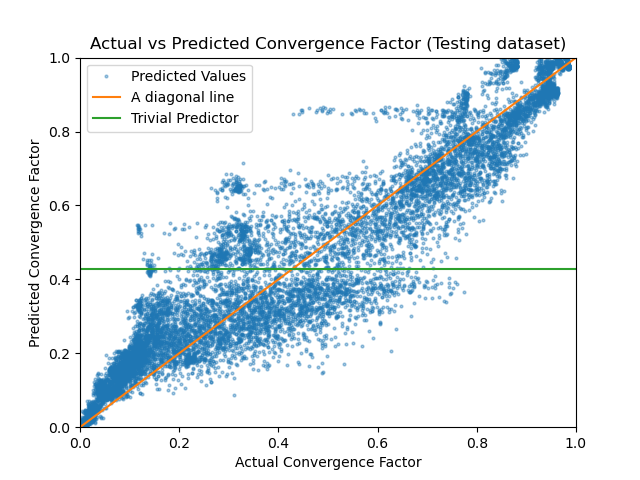
\includegraphics[width=\textwidth]{figs/cd_var_conv_mpnn_test_pred.png}
    \caption{Testing predictions}
    \label{subfig:cd_mpnn_test}
  \end{subfigure}
  \begin{subfigure}{.48\textwidth}
    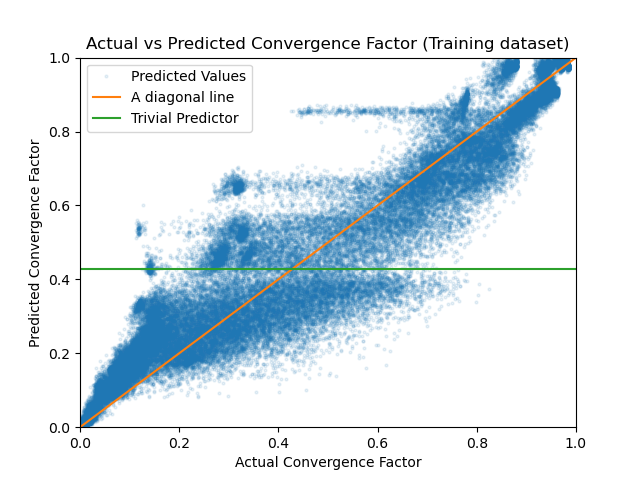
\includegraphics[width=\textwidth]{figs/cd_var_conv_mpnn_train_pred.png}
    \caption{Training predictions}
    \label{subfig:cd_mpnn_train}
  \end{subfigure}
  \caption{Predicted convergence rates vs. true convergence rates on (\ref{subfig:cd_mpnn_test}) testing and (\ref{subfig:cd_mpnn_train}) training datasets for model convection-diffusion problem, using an Edge-Conditioned Convolution network. Values closer to the diagonal represent more accurate predictions.}
  \label{fig:cd_mpnn_pred}
\end{figure}

\section{Discussion and Conclusions}\label{sec:conc}

In this paper, a method for training convolutional and graph nets was presented to predict convergence of a two-level multigrid solver when given an input C/F mesh splitting.  Random mesh splittings were generated from a set of reference grids for two model problems, then evaluated in a solver to find a reference convergence rate.  Additionally for the Poisson problem, a CNN to predict optimal relaxation weight was trained.

Results indicate that neural networks can indeed predict convergence for a multigrid solver.  Convolutional networks are effective at learning attributes on structured grid-like 1D or 2D meshes, and graph nets are able to generalize on variably-sized structured meshes.  The graph networks could be further developed and trained on more general classes of problems, instead of the specific convection-diffusion problem or the variable-coefficent Poisson equation.

Future works could build on the networks trained here and explore their applications, using them for example to pick between different AMG aggregation methods to find the most optimal for a specific use case.  Another more ambitious future work could be to use the neural networks in an optimization method to obtain the most convergent or most work efficient C/F splitting for a problem.

\bibliographystyle{siamplain}
\bibliography{references}

\end{document}
